%%%%%%%%%%%%%%%%%%%%%%%%%%%%%%%%%%%%%%%%%
% Beamer Presentation
% LaTeX Template
% Version 1.0 (10/11/12)
%
% This template has been downloaded from:
% http://www.LaTeXTemplates.com
%
% License:
% CC BY-NC-SA 3.0 (http://creativecommons.org/licenses/by-nc-sa/3.0/)
%
%%%%%%%%%%%%%%%%%%%%%%%%%%%%%%%%%%%%%%%%%

%----------------------------------------------------------------------------------------
%	PACKAGES AND THEMES
%----------------------------------------------------------------------------------------

\documentclass{beamer}

\mode<presentation> {

% The Beamer class comes with a number of default slide themes
% which change the colors and layouts of slides. Below this is a list
% of all the themes, uncomment each in turn to see what they look like.

%\usetheme{default}
%\usetheme{AnnArbor}
%\usetheme{Antibes}
%\usetheme{Bergen}
%\usetheme{Berkeley}
%\usetheme{Berlin}
%\usetheme{Boadilla}
%\usetheme{CambridgeUS}
%\usetheme{Copenhagen}
%\usetheme{Darmstadt}
%\usetheme{Dresden}
%\usetheme{Frankfurt}
%\usetheme{Goettingen}
%\usetheme{Hannover}
%\usetheme{Ilmenau}
%\usetheme{JuanLesPins}
%\usetheme{Luebeck}
%\usetheme{Madrid}
%\usetheme{Malmoe}
%\usetheme{Marburg}
%\usetheme{Montpellier}
%\usetheme{PaloAlto}
%\usetheme{Pittsburgh}
%\usetheme{Rochester}
\usetheme{Singapore}
%\usetheme{Szeged}
%\usetheme{Warsaw}

% As well as themes, the Beamer class has a number of color themes
% for any slide theme. Uncomment each of these in turn to see how it
% changes the colors of your current slide theme.

%\usecolortheme{albatross}
%\usecolortheme{beaver}
%\usecolortheme{beetle}
%\usecolortheme{crane}
%\usecolortheme{dolphin}
%\usecolortheme{dove}
%\usecolortheme{fly}
%\usecolortheme{lily}
%\usecolortheme{orchid}
%\usecolortheme{rose}
%\usecolortheme{seagull}
%\usecolortheme{seahorse}
%\usecolortheme{whale}
%\usecolortheme{wolverine}

%\setbeamertemplate{footline} % To remove the footer line in all slides uncomment this line
%\setbeamertemplate{footline}[page number] % To replace the footer line in all slides with a simple slide count uncomment this line

%\setbeamertemplate{navigation symbols}{} % To remove the navigation symbols from the bottom of all slides uncomment this line
}
\usepackage[english]{babel}
\usepackage[utf8x]{inputenc}
\usepackage{amsmath}
\usepackage{amsfonts}
\usepackage{amssymb}
\usepackage{graphicx} % Allows including images
\usepackage{booktabs} % Allows the use of \toprule, \midrule and \bottomrule in tables

%----------------------------------------------------------------------------------------
%	TITLE PAGE
%----------------------------------------------------------------------------------------
%<<<<<<< HEAD
%
\begin{document}

\title[K-Da Library]{K-Da Library} % The short title appears at the bottom of every slide, the full title is only on the title page
%
\author{Andrey Pérez Salazar\\ Andrés Sánchez López\\ David Pérez Bolaños} % Your name
\institute[UCR] % Your institution as it will appear on the bottom of every slide, may be shorthand to save space
{
University of Costa Rica \\ % Your institution for the title page
\medskip
%\textit{} % Your email address
}
\date{\today} % Date, can be changed to a custom date

%\begin{document}
%%%%%%%%%%%%%%%%%%%
\begin{frame}


\begin{figure}

\includegraphics[width=0.46\linewidth]{logo.jpg}
\end{figure}


\end{frame}

%%%%%%%%%%%%%%%%%%%
\begin{frame}
\frametitle{Review}
\begin{columns}[c] % The "c" option specifies centered vertical alignment while the "t" option is used for top vertical alignment

\column{.5\textwidth} % Left column and width
\begin{figure}
\centering
        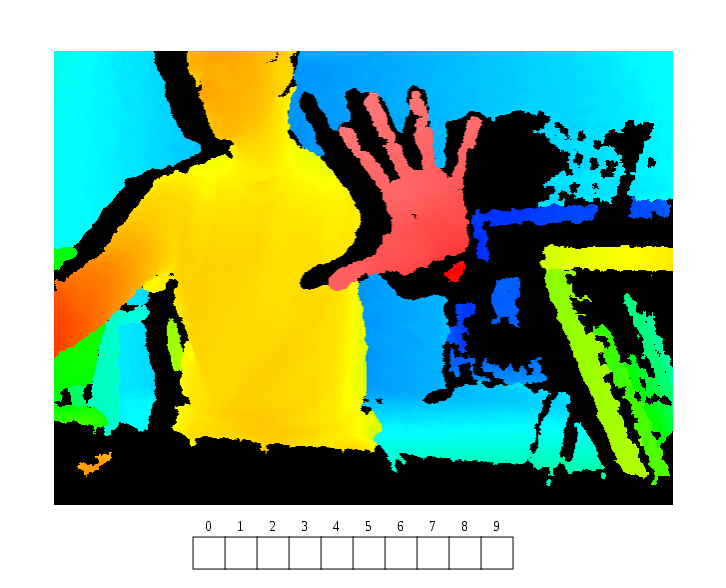
\includegraphics[totalheight=4.7cm]{kinect_array.png}
        %\includegraphics[width=0.8\textwidth]{bsp.eps}
    %\caption{imagen U.}
    \label{fig:verticalcell}
    \end{figure}

\column{.5\textwidth} % Right column and width
\begin{figure}
\centering
        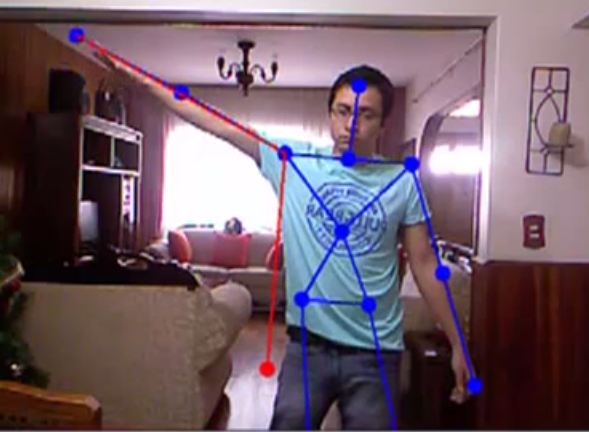
\includegraphics[totalheight=3.6cm]{comp2.png}
        %\includegraphics[width=0.8\textwidth]{bsp.eps}
    %\caption{imagen U.}
    \label{fig:verticalcell}
    \end{figure}

\end{columns}
\end{frame}


%%%%%%%%%%%%%%%%%%%%%
\begin{frame}
\frametitle{Problems of the previous presentation}
\begin{itemize}
\item Kinect-data\\~\\
\item Speed analysis
\end{itemize}

\end{frame}
%%%%%%%%%%%%%%%%%%%

\begin{frame}
\frametitle{Data structures to implement}

\begin{itemize}
\item Stack
\begin{figure}
\centering
        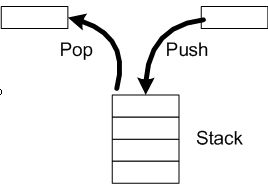
\includegraphics[totalheight=1.5cm]{Stack.jpg}
        %\includegraphics[width=0.8\textwidth]{bsp.eps}
    %\caption{imagen U.}
    \label{fig:verticalcell}
    \end{figure}
\item Double linked list
\begin{figure}
\centering
        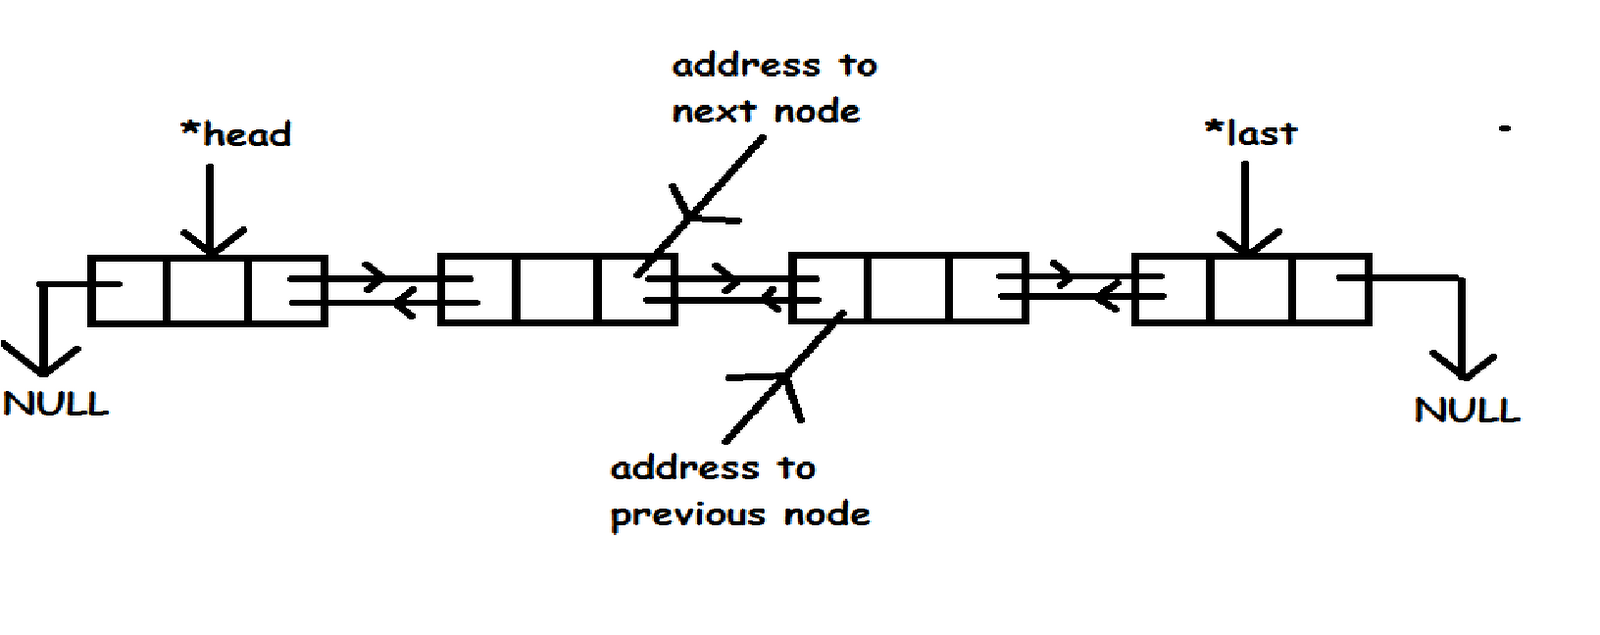
\includegraphics[totalheight=2cm]{list.png}
        %\includegraphics[width=0.8\textwidth]{bsp.eps}
    %\caption{imagen U.}
    \label{fig:verticalcell}
    \end{figure}
    
\item Queue

\begin{figure}
\centering
        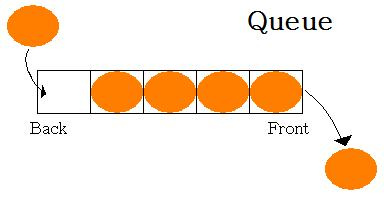
\includegraphics[totalheight=1.5cm]{queue.jpg}
        %\includegraphics[width=0.8\textwidth]{bsp.eps}
    %\caption{imagen U.}
    \label{fig:verticalcell}
    \end{figure}
\end{itemize}

\end{frame}

%%%%%%%%%%%%%%%%

\begin{frame}
\frametitle{Complexity Analysis}

\begin{center}
\begin{tabular}{l l   @{\hspace{1cm}}p{4cm}}
\cline{3-3}

\toprule
\textbf{Data Estructure} & \textbf{Storage} & \textbf{Using the methods} \\
\midrule
Stack & O(n) & O(n)\\
Linked list & O(1) & O(n)\\
Queue & O(1) & O(n)\\
\bottomrule
\end{tabular}
\end{center}

\end{frame}

%%%%%%%%%%%%%%%%%%%%%%%%%%%%

\begin{frame}

Class conversion
 
\begin{itemize}
\item convertir(string pjoint1, string pjoint2, int n);
\item llenarArregloAngulos();
\item getArregloAngulos();
\end{itemize}



\end{frame}
%%%%%%%%%%%%%%%%%%%%%%%%%%%%%%%

\begin{frame}

\begin{columns}[c] % The "c" option specifies centered vertical alignment while the "t" option is used for top vertical alignment

\column{0.4\textwidth}
 % Left column and width
\begin{figure}
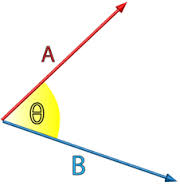
\includegraphics[width=0.45\linewidth]{punto.JPG}
\end{figure}

\column{.8\textwidth} % Right column and width

\begin{figure}
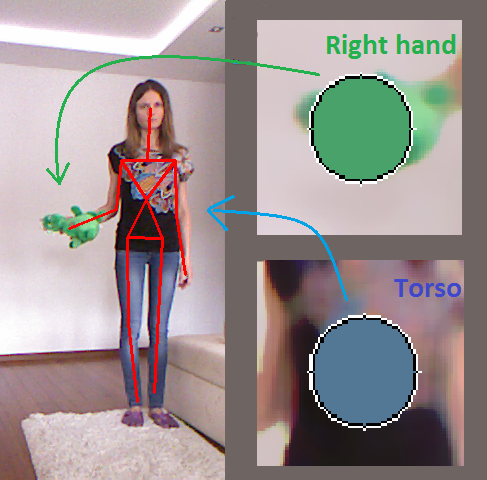
\includegraphics[width=0.7\linewidth]{conversion.png}
\end{figure}

\end{columns}

\begin{figure}
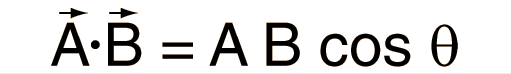
\includegraphics[width=0.5\linewidth]{prod_punto.png}
\end{figure}


\end{frame}


%----------------------------------------------------------------------------------------

\begin{frame}

Class compara
 
\begin{itemize}
\item sacapromedios(double arreglo);
\item arreglo\_promedio(double arreglo\_prom1, double arreglo\_prom2);

\end{itemize}

\end{frame}

%----------------------------------------------------------------------------------------

\begin{frame}

\begin{columns}[c] 

\column{.5\textwidth}
\textbf{sacapromedios}\\~\\

Array recibido:\\~\\
$\left[n,k,...,l,m\right.]$\\~\\~\\

Array retornado:\\~\\
$\left[prom(n,k,...,l,m)\right.]$

\column{.5\textwidth} % Right column and width

\textbf{arreglo\_promedio}\\~\\

Array recibido:\\~\\

$\left[prom(n1,k1,...,l1,m1)\right.]$\\~\\~\\
$\left[prom(n2,k2,...,l2,m2)\right.]$\\~\\~\\
Array retornado:\\~\\

$\left[1,0,0,1,0,1,1,0,1,1\right.]$

\end{columns}


\end{frame}

%----------------------------------------------------------------------------------------


\begin{frame}

Class compara
 
\begin{itemize}

\item comparar\_angulos(int promedio);
\item comparar\_velocidad(int pSizeMov1, int pSizeMov2);
\end{itemize}

\end{frame}

%----------------------------------------------------------------------------------------

\begin{frame}


\begin{columns}[c] % The "c" option specifies centered vertical alignment while the "t" option is used for top vertical alignment

\column{.5\textwidth}
 % Left column and width
\begin{figure}
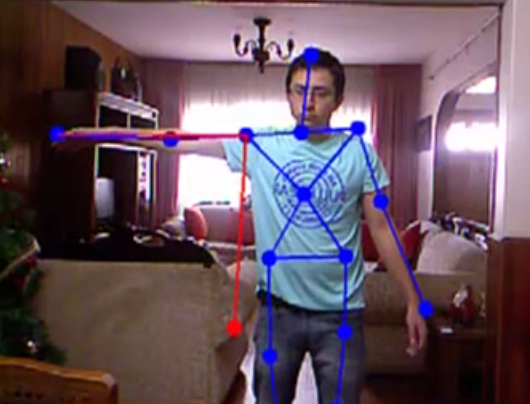
\includegraphics[width=0.9\linewidth]{comp1.png}
\end{figure}

\column{.5\textwidth} % Right column and width

\begin{figure}
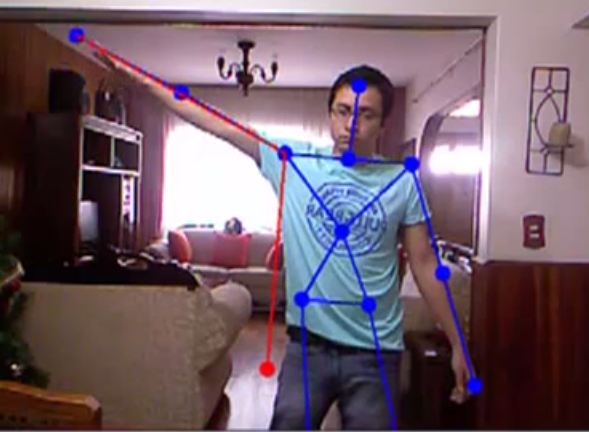
\includegraphics[width=0.9\linewidth]{comp2.png}
\end{figure}

\end{columns}



\end{frame}
%----------------------------------------------------------------------------------------

\begin{frame}


\begin{figure}
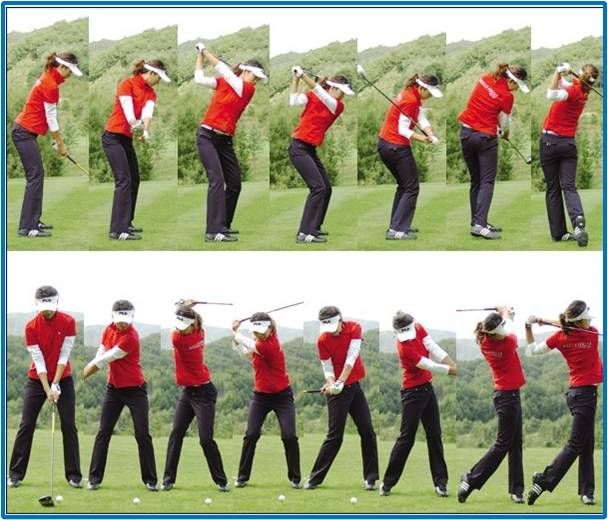
\includegraphics[width=0.76\linewidth]{frames.jpg}
\end{figure}


\end{frame}
%----------------------------------------------------------------------------------------
\begin{frame}


Gracias

%----------------------------------------------------------------------------------------
\end{frame}

\end{document} 
